\subsection{Stream Partitioning}
We use the Geohash~algorithm~\cite{geohash} to balance load and partition incoming data streams across processing resources. Geohash divides the earth into a hierarchy of bounding boxes identified by Base 32 strings; the longer the Geohash string, the more precise the bounding box. Figure~\ref{fig:geohash} illustrates this hierarchy. Most of the eastern United States is contained within the bounding box described by Geohash string \emph{D}, while \emph{DJ} encompasses substantial parts of Florida, Georgia, and Alabama. The bounding box \emph{DJKJ} (highlighted in red) contains Tallahassee, Florida. This hierarchical representation enables \textsc{Synopsis} to cope with both low- and high-density regions: several resources may be tasked with managing streams originating in and around large cities, while rural areas fall under the purview of a single node.

\begin{figure}[b!]
    \centerline{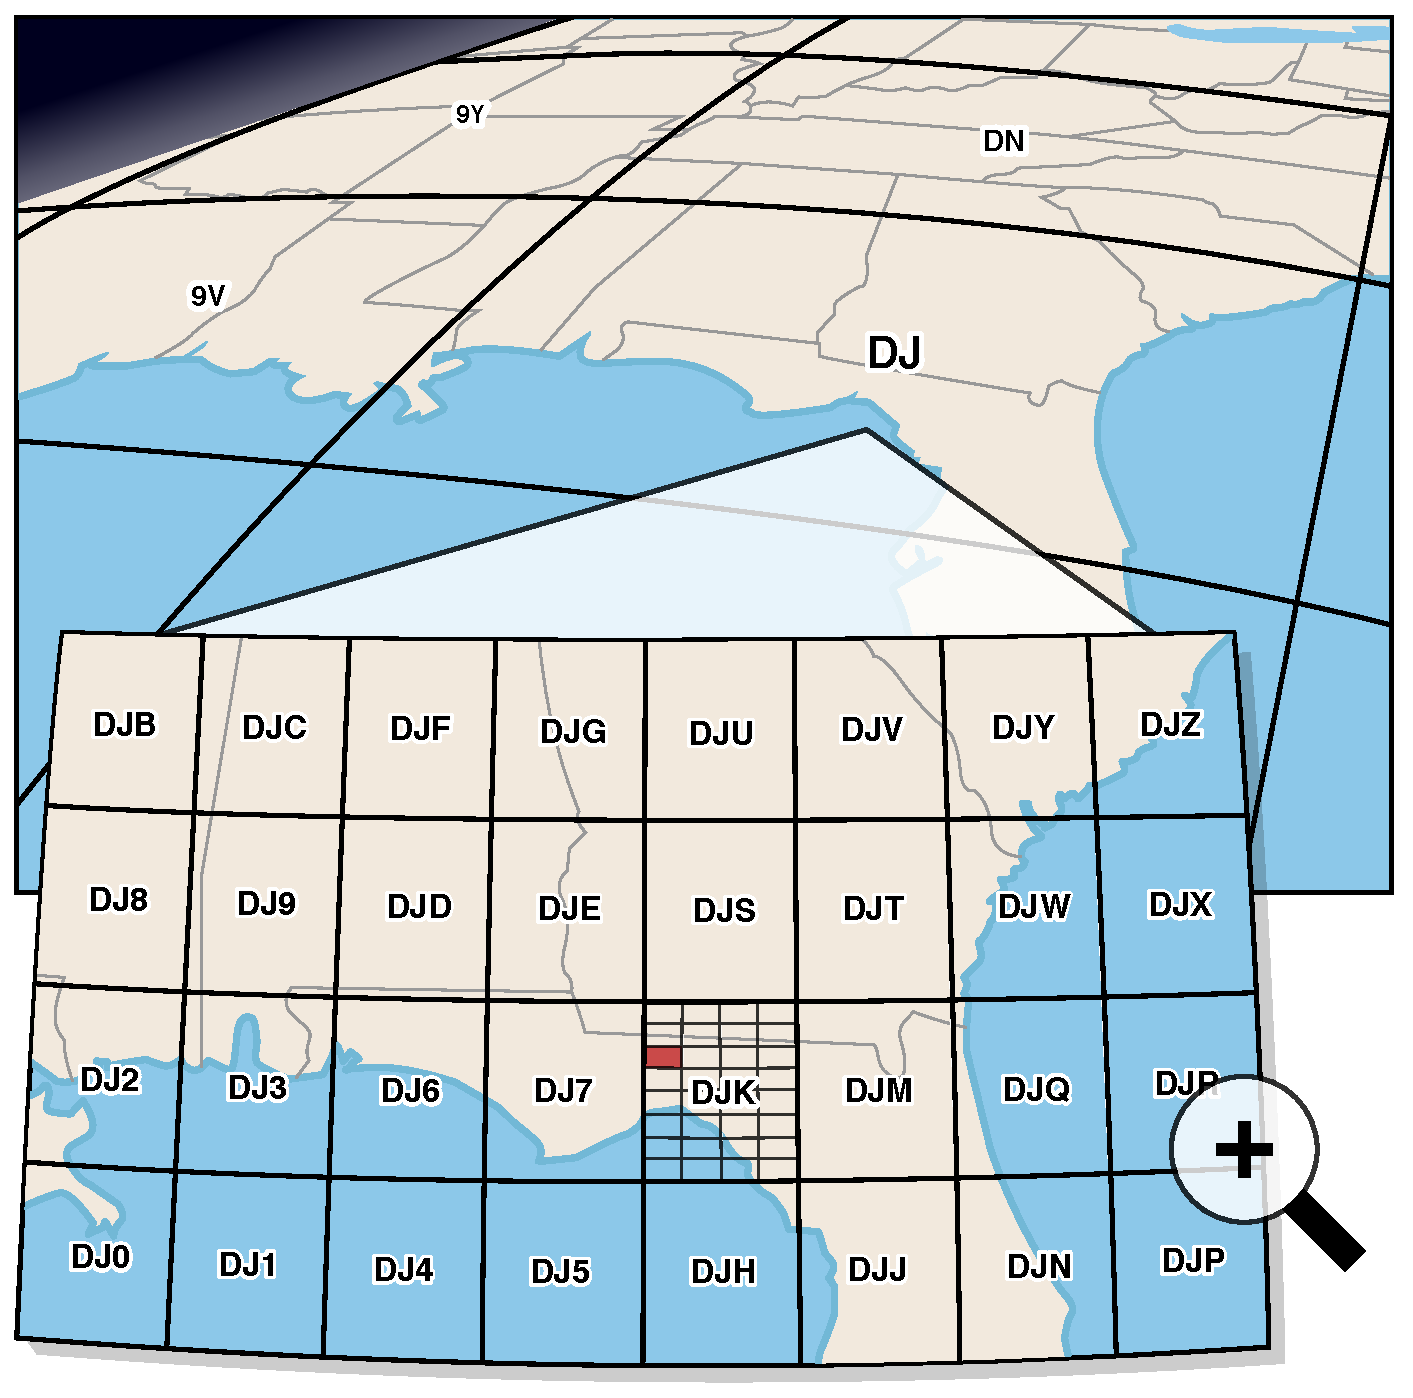
\includegraphics[width=3.5in]{figures/geohash.pdf}}
    \caption{A demonstration of the Geohash algorithm. Each additional character in a Geohash string describes a finer-grained region; Geohash \emph{DJ} contains substantial parts of Florida, Georgia, and Alabama, USA, while \emph{DJKJ} (highlighted in red) encompasses Tallahassee, the capital of Florida.}
    \label{fig:geohash}
\end{figure}

To achieve fine-grained control over our Geohash partitions, we operate at the bit level rather than Base 32 character level when routing streams. Each bit added to a Geohash string reduces its scope by half, with each character represented by five bits ($2^5 = 32$). In other words, a four-character Geohash string represents 20 spatial subdivisions applied recursively to each resulting region. This property allows us to manage and allocate resources across a wide variety of observational densities.

Figure~\ref{fig:stream-partitioning} depicts a possible arrangement of the distributed sketch and the associated stream partitioning scheme corresponding to our example region.
The distributed sketch is arranged in a tree-like structure.
Stream ingesters act as root nodes of the tree and partition the stream among \textsc{Synopsis} nodes using a Geohash-based partitioning function.
Nodes closer to the root hold sketches corresponding to shorter Geohash strings, and therefore larger geographical regions.
For instance, nodes A and B in Figure~\ref{fig:stream-partitioning} are responsible for regions represented by Geohashes \emph{DJ} and and \emph{DN} respectively.
Node E, which is three edges deep from the stream ingester, is responsible for a smaller region, \emph{DJKJ}.

\textsc{Synopsis} is designed to ensure that regions corresponding to larger portions of the input streams (hence, more frequent updates) are moved to dedicated or less crowded nodes.
If a node decides to scale out a portion of the region it is currently responsible for, then the corresponding state (sketchlet and related metadata) is transferred over to the new computation and it starts to treat the stream packets corresponding to the scaled out region as pass-through traffic (Scaling out is explained in section~\ref{subsec:scaling-out}).
More specifically, the node will not process the stream packet, but instead updates its statistics based on the headers of the packet and forwards it to the destination child node. 
For instance, node A in Figure~\ref{fig:stream-partitioning} has scaled out two regions (\emph{DJK} and \emph{DJM}) to nodes C and D.
After these two scaling out operations, node A is responsible for all sub-regions in \emph{DJ} except for \emph{DJK} and \emph{DJM}.
Similarly, the sketch for the region \emph{DJKJ} is moved out of node C into node E as a result of subsequent scale out operation.
It should be noted that the depth and span of the distributed sketch are dynamic and are constantly evolving according to the workload and operating conditions.

As the tree grows, having parent nodes pass traffic through to their children becomes inefficient because of higher bandwidth consumption as well as increased latency due to additional network hops the packets have to travel through.
To circumvent this, we allow \emph{short circuiting}, which directs traffic from stream ingesters straight to child nodes.
This is depicted in Figure~\ref{fig:stream-partitioning}, where the stream ingester directly sends data to node E instead of sending it through nodes A and C.
We use our gossiping subsystem to update parent nodes on child state information, which is useful for scaling in as explained in Section~\ref{subsec:scaling-in}.

\begin{figure}
    \centerline{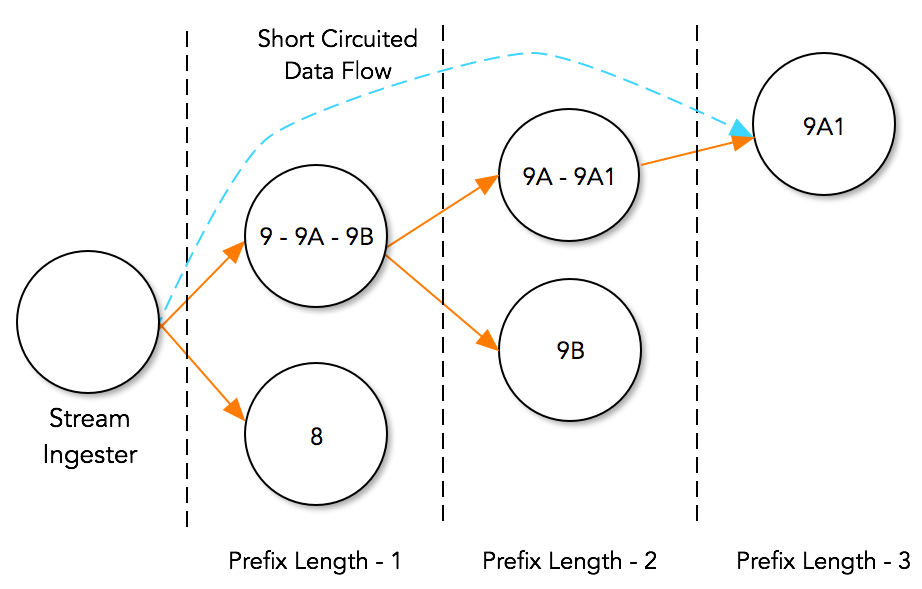
\includegraphics[width=3.5in]{figures/stream-partitioning.png}}
    \caption{An example of our stream partitioning approach based on the Geohash values of incoming packets.}
    \label{fig:stream-partitioning}
\end{figure}
